% Word Count Comparison Chart
% Add to main.tex after \begin{document}

\begin{figure}[t]
\centering
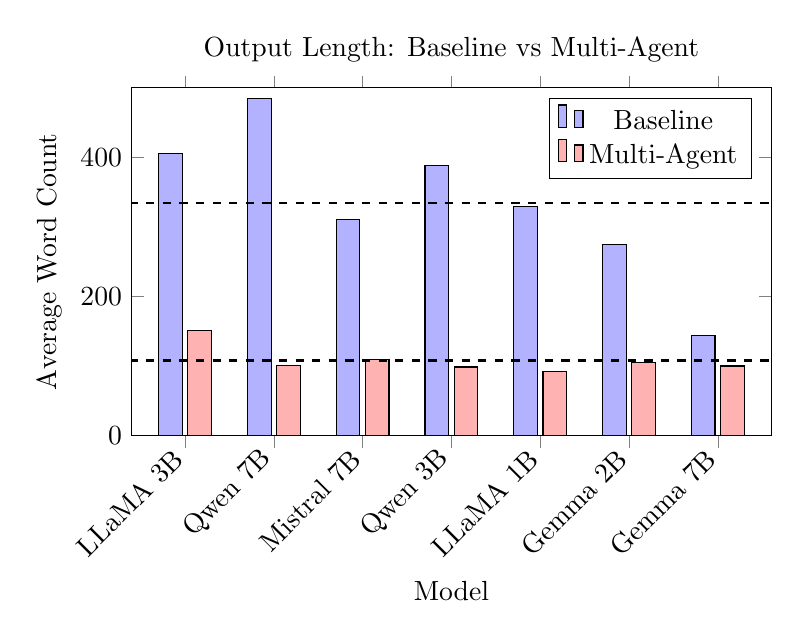
\begin{tikzpicture}
\begin{axis}[
    width=0.8\textwidth,
    height=6cm,
    ybar,
    bar width=0.3cm,
    xlabel={Model},
    ylabel={Average Word Count},
    ymin=0, ymax=500,
    xtick={1,2,3,4,5,6,7},
    xticklabels={LLaMA 3B, Qwen 7B, Mistral 7B, Qwen 3B, LLaMA 1B, Gemma 2B, Gemma 7B},
    x tick label style={rotate=45, anchor=east},
    legend pos=north east,
    title={Output Length: Baseline vs Multi-Agent}
]

% Baseline word counts
\addplot[fill=blue!30] coordinates {
    (1, 405.9)
    (2, 484.3)
    (3, 310.2)
    (4, 389.0)
    (5, 329.3)
    (6, 275.2)
    (7, 144.7)
};

% Multi-agent word counts
\addplot[fill=red!30] coordinates {
    (1, 150.9)
    (2, 100.4)
    (3, 109.8)
    (4, 98.9)
    (5, 92.6)
    (6, 105.0)
    (7, 100.3)
};

\legend{Baseline, Multi-Agent}

% Average line
\draw[dashed, thick, black] (axis cs:0,334.1) -- (axis cs:8,334.1);
\node[right] at (axis cs:7.5,334.1) {Baseline Avg: 334.1};

\draw[dashed, thick, black] (axis cs:0,108.3) -- (axis cs:8,108.3);
\node[right] at (axis cs:7.5,108.3) {Agent Avg: 108.3};

\end{axis}
\end{tikzpicture}
\caption{Output length comparison between baseline and multi-agent architectures. Multi-agent outputs are 67.6\% shorter on average (108.3 vs 334.1 words) while achieving higher ROUGE scores.}
\label{fig:wordcount}
\end{figure}
